\chapter[Scarefault]{Scarefault}
Neste capítulo será abordado o \Scarefault, o produto final desse
trabalho. Este capítulo está dividido em seções. A primeira seção aborda
uma visão geral do \Scarefault. A segunda seção faz uma análise da
arquitetura do \framework e suas dependências. Na seção seguinte explana-se
a respeito da utilização do \Scarefault.

\section{\Scarefault: Visão Geral}
O \scarefault é um \framework que tem a intenção de gerar testes unitários
de forma semiautomatizada. Para isso, ele necessita da intervenção do
desenvolvedor que o utiliza por meio de breves especificações nos
comentários de documentação. A partir dessas especificações o \scarefault
coleta informações necessárias para a produção dos casos de teste e gera
um arquivo contendo os testes solicitados. É importante ressaltar que,
para esse trabalho, os testes gerados são apenas testes caixa preta.

O \framework se propõe em permitir a acoplagem de diferentes linguagens
de programação. Para isso, há a necessidade da construção de um \parser
que identifique a sintaxe da linguagem alvo por meio de duas
ferramentas: \flexcpp e \textsf{Bisonc++}. Essas duas ferramentas são
comuns em contextos de produção de compiladores. Com o \parser
implementando o desenvolvedor poderá implementar as especificidades
relacionadas aos testes da linguagem alvo, tendo como base o código
oferecido pelo \Scarefault.

O \scarefault foi escrito em \cpp e está licenciado dentro das condições
da \textsf{GPLv3}. Todo o seu código fonte encontra-se em:
\url{https://github.com/Scarefault/scarefault}.

\section{A Arquitetura do \scarefault}
Essa seção evidencia os elementos da arquitetura do \Scarefault. Como
ele foi desenhado, quais conceitos foram utilizados e como ele funciona.
Em um primeiro momento são exploradas visões estáticas da arquitetura.
A visão dinâmica da arquitetura é melhor evidenciada pela seção seguinte.

\subsection{Visão de Pacotes}
Partindo-se de uma visão macroscópica, o \scarefault pode ser dividido em
dois módulos básicos: o \textsf{identifier} e o \textsf{generator}. A Figura
\ref{modules-scarefault} ilustra esses módulos básicos.

\begin{figure}[h]
  \centering
    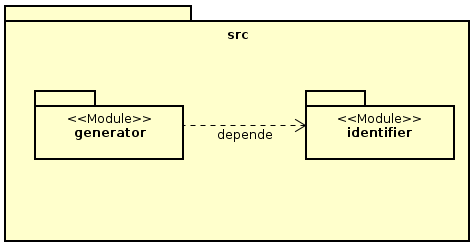
\includegraphics[width=0.6\textwidth]{figuras/modules-scarefault.png}
    \caption{Representação dos módulos do \Scarefault}
    \label{modules-scarefault}
\end{figure}
\FloatBarrier

\begin{description}
\item[identifier:] é responsável pela identificação das regras que regem
a gramática da linguagem de programação alvo, bem como da coleta dos dados
necessários para a produção dos casos de teste.
\item[generator:] responsável pela geração dos casos de teste. A partir dos dados
coletados das especificações do desenvolvedor e do próprio código fonte, esse
módulo é capaz de gerar casos de teste.
\end{description}

Expandindo-se os módulos pode-se observar os pacotes associados a cada um deles
e o relacionamento entre esses pacotes, como mostra a Figura
\ref{expand-modules-scarefault-1}.

\begin{figure}[h]
  \centering
    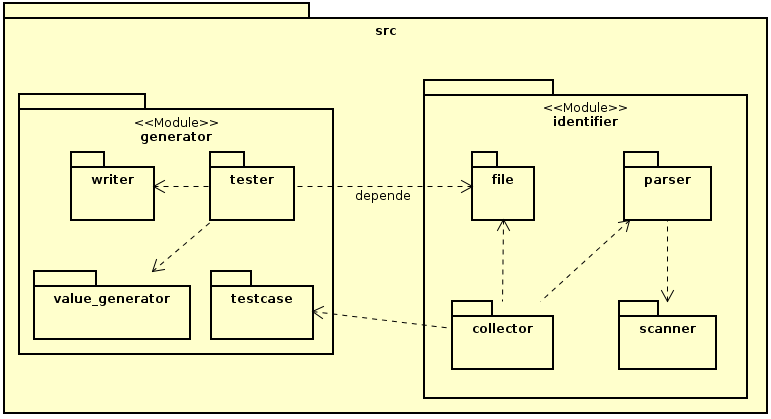
\includegraphics[width=0.8\textwidth]{figuras/expand-modules-scarefault-1.png}
    \caption{Representação expandida dos módulos do \Scarefault}
    \label{expand-modules-scarefault-1}
\end{figure}

Como indicado na Figura \ref{expand-modules-scarefault-1}, os pacotes associados ao
módulo \textsf{identifier} são:
\begin{description}
\item[\textit{scanner}:] responsável pela análise léxica do arquivo contendo o código
fonte em avaliação. As classes contidas nesse pacote são geradas pelo \flexcpp durante
a compilação.
\item[\textit{parser}:] responsável pela análise sintática do arquivo contendo o
código em avaliação. As ações que ele executa quando determinada regra gramatical é
encontrada são, essencialmente, ações de coleta de dados. As classes associadas
a esse pacote são geradas pelo \bisoncpp durante a compilação.
\item[\textit{collector}:] responsável pela coleta de dados necessários para a
criação de testes unitários.
\item[\textit{file}:] responsável por guardar os dado coletados do código fonte.
Dados como as dependências (\textit{libraries} importadas), métodos e classe
do arquivo em análise.
\end{description}

Os pacotes associados ao módulo \textsf{generator}, como mostra a Figura
\ref{expand-modules-scarefault-1}, são:
\begin{description}
\item[	\textit{tester}:] responsável pela construção dos arquivos de teste. A partir
dele é que os testes ganham forma, conforme a linguagem de programação.
\item[	\textit{testecase}:] responsável por guardar os dados relacionados
a cada caso de teste especificado pelo desenvolvedor, a partir dos
comentários no código fonte.
\item[	\textit{value\_generator}:] responsável por gerar valores randômicos
para o desenvolvimento dos testes.
\item[\textit{writer}:] responsável por escrever as informações da arquivo de
teste, enviadas pelo \textsf{tester}. Para isso, ele cria o arquivo e
escreve todas as informações a ele solicitadas.
\end{description}

\subsection{Visão de Classes}
As Figuras \ref{modules-scarefault} e \ref{expand-modules-scarefault-1} mostram
a visão de pacotes do \scarefault e como eles se relacionam, bem como a
responsabilidade que cabe a cada um deles. Aprofundando-se mais, chega-se a uma
visão das entidades associadas a cada pacote. A visão de quais são essas
entidades e como elas se relacionam pode ser verificada pelo diagrama de 
domínio, mostrado na Figura \ref{domain-diagram}.
\begin{figure}[h]
  \centering
    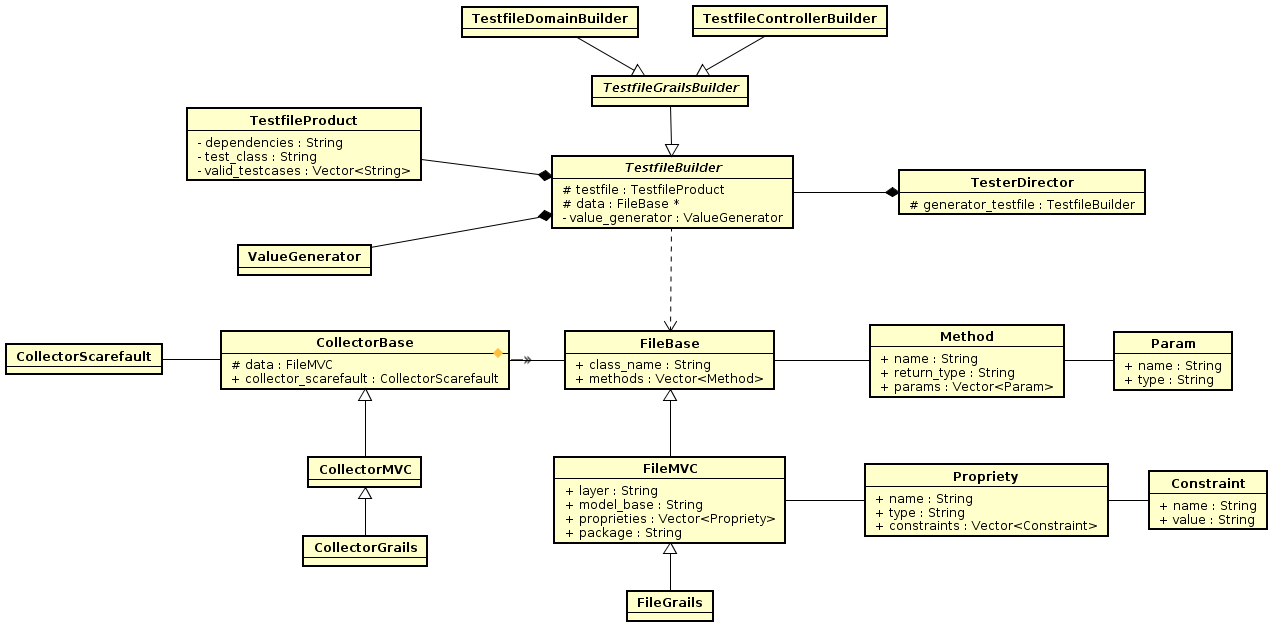
\includegraphics[width=\textwidth]{figuras/domain-diagram.png}
    \caption{Diagrama de domínio do \Scarefault}
    \label{domain-diagram}
\end{figure}
\FloatBarrier

O diagrama de domínio na Figura \ref{domain-diagram} demonstra a relação
entre as principais entidades que o \framework trabalha. O \textsf{Collector}
recolhe as  informações essencias para os testes a partir do
\textsf{Parser} que, por sua vez, recebe um \textit{stream} de dados a partir
do \textsf{Scanner}. Como dados importantes para a produção de testes pelo
\scarefault tem-se métodos (\textsf{Method}) e seus parâmetros (\textsf{Param})
e, para arquiteturas voltadas ao MVC, tem-se propriedades (\textsf{Propriety})
e suas restrições (\textsf{Constraint}). Esses dados estão intimamente ligados
ao arquivo em análise, portanto, são armazenados na entidade arquivo (\textsf{FileBase}).
Há também a entidade \textsf{TestCase} que tem papel fundamental na produção
dos testes, pois carrega as informações dispostas pelo desenvolvedor sobre os
testes a serem criados. Uma parte importante dos casos de teste são os
argumentos (\textsf{Arg}) que devem ser passados ao método em avaliação durante o
teste.

Partindo-se do diagrama de domínio exposto na Figura \ref{domain-diagram}, pode-se
visualizar o diagrama de classe, mostrado na Figura \ref{class-diagram}.
%\begin{landscape}
\begin{figure}[h]
  \centering
    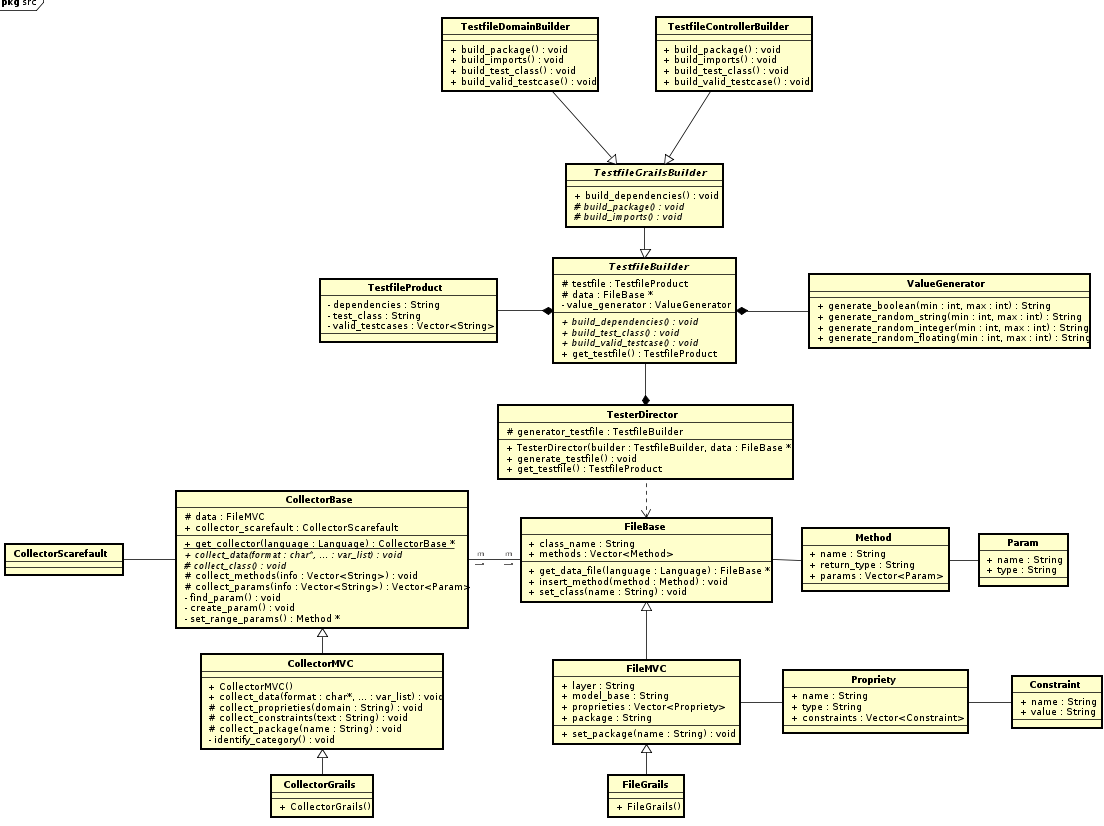
\includegraphics[width=\textwidth]{figuras/class-diagram.png}
    \caption{Diagrama de classe completo do \Scarefault}
    \label{class-diagram}
\end{figure}
\FloatBarrier
%\end{landscape}

O diagrama de classes permite obter uma visualização mais apurada dos
relacionamentos entre as classes contidas no \textit{framework}. As principais
entidades do \textit{framework}, apresentadas na Figura \ref{domain-diagram},
estão presentes e muitas delas passaram a ter um conjunto auxiliar de classes,
de forma a permitir a sua adaptação ao contexto em que será inserida.

Por meio da Figura \ref{class-diagram} pode-se identificar o uso de alguns
\textit{design patterns} de criação, com o intuito de permitir a
extensibilidade do \framework e a sua facilidade de uso. Para esse fim,
foram usados os conceitos do \textbf{\textit{builder pattern}} e
\textbf{\textit{factory pattern}}.

\subsubsection{\textit{Builder Pattern}}
O uso do \textit{builder pattern} vem para solucionar um problema
na criação de objetos complexos. Seu intuito é a separação do processo
de construção da representação em si. Desse modo, é possível que o
mesmo processo de construção sirva para diferentes representações
\cite{gammaEtAl1994}.

No desenvolvimento do \framework observou-se essa necessidade na
criação de objetos \textsf{Testfile}. Essa entidade é diferente para
cada linguagem associada a ele. Não é possível manter uma mesma
representação desse objeto, no entanto, o processo de criação de um
\textsf{Testfile} é igual em todos os casos: escreve-se as
dependências da classe de teste, o cabeçalho da classe de teste,
as ações iniciais para os testes (\textit{setup}),
os casos de teste, as ações para depois de cada teste
(\textit{teardown}) e a finalização do arquivo.

Nesse sentido, viu-se a solução proposta pelo \textit{builder pattern}
como saída para o problema dentro do contexto do desenvolvimento do
\Scarefault. A Figura \ref{testfile-diagram} mostra como a solução
foi desenhada.
\begin{figure}[h]
  \centering
    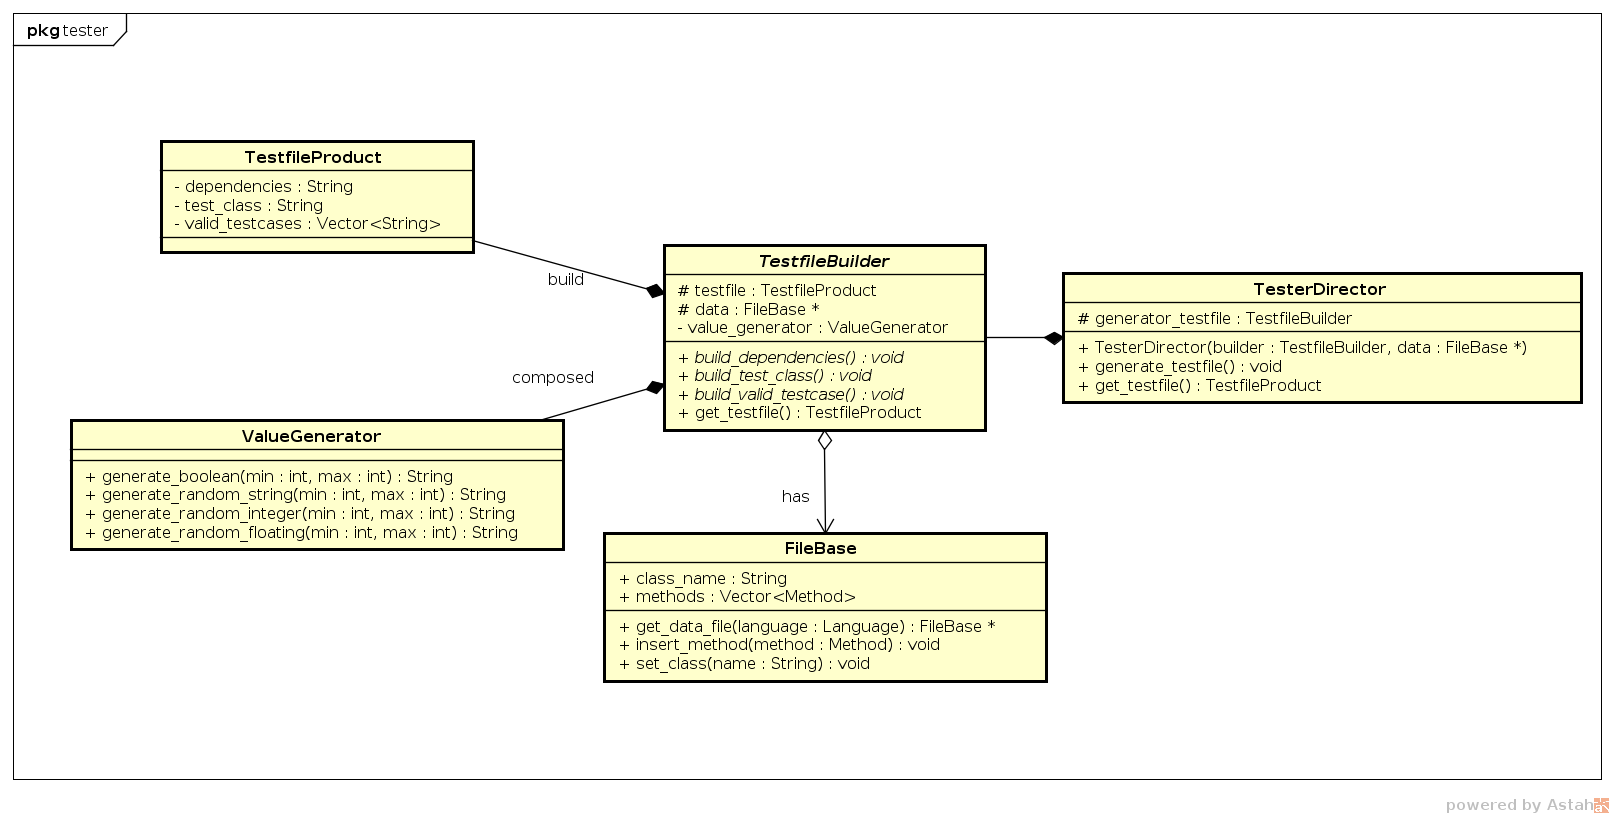
\includegraphics[width=\textwidth]{figuras/testfile-diagram.png}
    \caption{Diagrama de classes apresentando o \textit{builder pattern} no \framework}
    \label{testfile-diagram}
\end{figure}
\FloatBarrier

O objeto a ser construído é da classe \textsf{TestfileProduct}. Há
diversas representações que esse objeto pode tomar, conforme a linguagem.
No entanto, o processo de construção é o mesmo. Os passos desse processo são definidos
pela classe \textsf{TestfileBuilder}. Essa classe é uma classe
\textsf{virtual} (abstrata). Ela define uma interface que deve ser
implementada pelas suas classes filhas, afim de construir o objeto
\textsf{TestfileProduct}. Dessa forma, garante-se que qualquer
classe com a responsabilidade de construir um \textsf{TestfileProduct}
terá funções-membro que criem os elementos essenciais do produto. Com a garantia
que os passos de construção estão implementados, pode-se fazer o processo de
criação. Essa atividade é responsabilidade do \textsf{TesterDirector}. O
método \lstinline|generate_testfile()| possui a definição do processo de
construção, a partir dos passos estipulados pelo \textsf{TestfileBuilder}.

\subsubsection{\textit{Factory Pattern}}
\textit{Facotry pattern} é uma solução pensada com o propósito de deixar a
instanciação de objetos de uma mesma família mais flexível. Através desse
padrão  é possível instanciar um objeto sem expor a lógica dessa ação, bem
como ser capaz de referenciar-se a novos objetos por uma interface comum
\cite{gammaEtAl1994}.

No construção do \scarefault deparou-se com a necessidade de flexibilizar
a instanciação de objetos de coleta de dados. Isso fornece maior liberdade
ao desenvolvedor usuário do \framework para criar suas próprias classes de
coleta, que estarão relacionadas a uma determinada linguagem de programação
e suas peculiaridades.

Por esse motivo foi pensado no \textit{Factory pattern} como solução. A Figura
\ref{collector-diagram} mostra a solução desenhada para o \textit{framework}.
\begin{figure}[h]
  \centering
    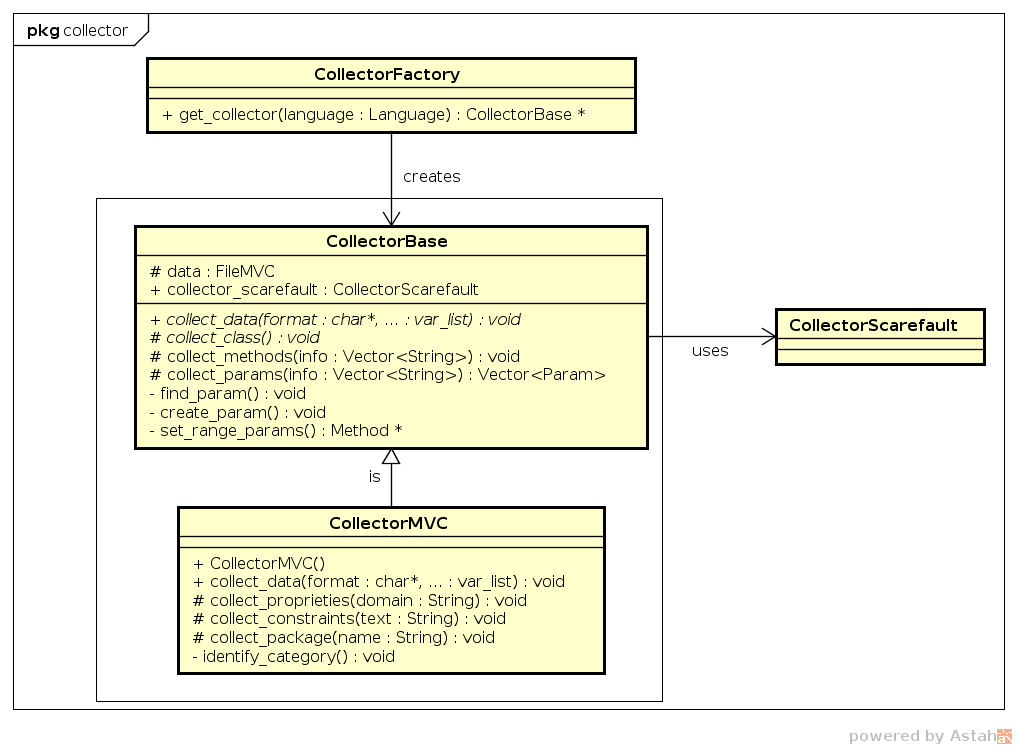
\includegraphics[width=\textwidth]{figuras/collector-diagram.png}
    \caption{Diagrama de classes apresentando o \textit{factory pattern} no \framework}
    \label{collector-diagram}
\end{figure}
\FloatBarrier

A solução de \textit{factory pattern} desenvolvida utiliza-se de uma classe
\textsf{virtual} denominada \textsf{CollectorBase}. Optou-se por uma classe
desse tipo, ao invés de uma \textsf{virtual} pura (\textsf{interface}), pois
imaginou-se em já deixar implementadas determinadas funções-membro auxiliares,
preparadas para serem usadas pelo usuário. Essas funções-membro, embora já implementadas,
são passíveis de sobreescrita, o que dá a possibilidade do desenvolvedor
decidir criar as sua própria forma de coletar determinados elementos ou utilizar-se
da já disponível.

A única função-membro obrigatória de implementação para as classes derivadas da
\textsf{CollectorBase} é a \lstinline|collect_data(char *, ...)|. Além disso, já
há uma outra classe de coleta preparada para linguagens que se utilizem do padrão
de projeto MVC: a \textsf{CollectorMVC}. Ela também extende a \textsf{CollectorBase},
mas traz outras funções-membro auxiliares.

A classe \textsf{CollectorFactory} é reponsável por esconder a lógica de instanciação
da família \textit{Collector}. Por meio da \lstinline|get_collector()| um objeto
\textsf{CollectorFactory} retorna uma instância do \textit{Collector} solicitado na
classe cliente.

\section{A Utilização do \Scarefault}
A utilização do \scarefault pode ser dividida em dois objetivos: a adaptação do \textit{framework} para atender uma nova linguagem e a geração de testes unitários.
 
\subsection{Adaptação para uma Nova Linguagem}
A adaptação do \scarefault para novas linguagens exige o uso de um ambiente específico de desenvolvimento, bem como o uso de janelas de extensibilidade do \textit{framework}, chamadas de \textit{hotspots}.

\subsubsection{Usando o Ambiente de Desenvolvimento}
Para auxiliar na customização do \textit{framework}, criou-se um ambiente virtual de forma a garantir a instalação das dependências necessárias do \Scarefault. Para levantar esse ambiente é necessário que o usuário instale as versões mais recentes das seguintes ferramentas: 

\begin{description}
\item[Git:] ferramenta de controle de versão;
\item[VirtualBox:] ferramenta de virtualização de máquinas virtuais;
\item[Vagrant:] ferramenta de criação e configuração de ambientes virtuais de desenvolvimento.
\end{description} 


Com essas ferramentas instaladas, o usuário deve efetuar o clone do projeto e executar o comando responsável por criar o ambiente virtual com as configurações predefinidas. Nesse momento será instalado e configurado o \textsf{Flexc++}, \textsf{Bisonc++} e demais dependências. Por fim, deve-se acessar essa máquina virtual e então iniciar a customização no código do \Scarefault. O Código \ref{ambientevirtual} apresenta as linhas de comando referentes aos passos citados:

\begin{lstlisting}[language=make, label=ambientevirtual, caption=Levantamento do Ambiente de Desenvolvimento]
git clone git@github.com:Scarefault/scarefault.git
cd scarefault
vagrant up
#Aguarde instalação e configuração das dependências
vagrant ssh
\end{lstlisting}

O \scarefault contempla a linguagem de programação \grails até o momento. Para facilitar a compilação do \Scarefault, criou-se um \textsf{Makefile} responsável por fazer o \textit{build}. Isso se fez necessário porque a compilação dos arquivos-fonte exige um linha de comando extensa. Além disso, há algumas alterações fundamentais a serem feitas em determinados arquivos para que se faça a comunicação entre o \scanner e o \textsf{parser}.

\subsubsection{Explorando a Extensibilidade do \Scarefault}
O \scarefault por si só não é uma aplicação. Nesse sentido, ele precisa ter determinados pontos extendidos para que possa ser executado. Essencialmente, o \scarefault permite a acoplagem de novas linguagens. Para isso, há alguns pontos de extensão para que isso ocorra. São eles: adição de um \parser para a nova linguagem, criação do agente de coleta de dados e do agente de construção de casos de teste.

O \parser é desenvolvido utilizando o \textsf{Flexc++} e o \textsf{Bisonc++}. Para uso dessas ferramentas, recomenda-se o uso da documentação oficial, disponível em \url{https://fbb-git.github.io/flexcpp/} e \url{https://fbb-git.github.io/bisoncpp/}, respectivamente. Após a gramática da nova linguagem ter sido criada



\subsection{Geração de Testes Unitários}


